Das Generic Access Profile (GAP) definiert verschiedene Rollen und Modi bzw. Prozeduren für Broadcasts und den Aufbau von Verbingungen.

Für LE existieren die vier Rollen: Broadcaster, Observer, Peripheral und Central. Ein Broadcaster ist aus Sicht des Link Layers (LL) ein Advertiser, da er verbindungslos Daten in Form von Advertising Events sendet. Der zugehörige Modus ist der Broadcast Mode. Diese Advertising Events können von Observern, die die Observation Procedure ausführen, empfangen werden, weswegen diese aus Sicht des LL als Scanner bezeichnet werden. Die Rolle Peripheral wird einem Gerät zugewiesen, wenn es den Aufbau eines LE Physical Link akzeptiert. Dabei nimmt es in Bezug auf den Link Layer die Rolle des Slave ein. Die Rolle Central wird einem Gerät zugewiesen, wenn dieses den Aufbau einer physischen Verbindung einleitet. Dabei nimmt es in Bezug auf den Link Layer die Rolle des Master ein. Ein Gerät kann mehrere Rollen zur selben Zeit einnehmen. \cite{BtSpec4.0_1638-1639} \cite{BtSpec4.0_1695-1697}
% QUELLE Spec 4.0 S. 1638 f. 2.2.2 Roles when Operating over an LE Physical Channel
% QUELLE Spec 4.0 S. 1695 f. 9.1

Jedes Gerät befindet sich entweder im Non-discoverable Mode, in dem es nicht von anderen Geräten entdeckt werden kann, oder im General Discoverable Mode bzw. im Limited Discoverable Mode, in denen es entdeckbar ist. Im Letzteren ist ein Gerät nur für eine bestimmte Dauer entdeckbar. Geräte, die andere Geräte entdecken sollen, müssen die General Discovery Procedure bzw. Limited Discovery Procedure ausführen. \cite{BtSpec4.0_1697}
% QUELLE Spec 4.0 S. 1697 9.2 Discovery Modes And Procedures

Um Verbindungen und deren Aufbau zu steuern, gibt es mehrere Modi und Prozeduren, von denen einige in der Tabelle X zusammengefasst werden.
% TODO TABELLE VERWEIS

\begin{table}
    \begin{tabularx}{\textwidth}{|p{4.5cm}|X|}
    \hline
    \textbf{Modus/Prozedur} & \textbf{Beschreibung} \\
    \hline
    Non-connectable Mode & keine Verbindungen akzeptieren \\
    \hline
    Directed Connectable Mode & nur Verbindungen von bekannten Peer-Geräten (Bluetooth-Adresse bekannt) akzeptieren, die die Auto oder General Connection Establishment Procedure ausführen \\
    \hline
    Undirected Connectable Mode & nur Verbindungen von Geräten akzeptieren, die die Auto oder General Connection Establishment Procedure ausführen \\
    \hline
    Auto Connection Establishment Procedure & Aufbau von Verbindungen zu Geräten, die in einem Connectable Mode sind und deren Adresse auf der Whitelist eingetragen ist \\
    \hline
    General Connection Establishment Procedure & Aufbau von Verbindungen zu bekannten Peer-Geräten, die in einem Connectable Mode sind \\
    \hline
    Connection Parameter Update Procedure & Peripheral oder Central kann Link-Layer-Parameter einer Verbindung ändern \\
    \hline
    \end{tabularx}
    \caption[Modi und Prozeduren für Verbindungen (GAP)]{Modi und Prozeduren für Verbindungen \cite{BtSpec4.0_1704-1718}}
\end{table}
% QUELLE Spec. 4.0 S. 1704 - 1718 9.3 Connection Modes and Procedures

Bonding ist das Speichern von Sicherheits- und Identitätsinformationen wie dem Identity Resolving Key (IRK) oder dem Long Term Key (LTK). Der IRK generiert zufällige Adressen oder löst diese auf. Der LTK wird beim Pairing generiert und dient zur Verschlüsselung einer Verbindung (siehe Sektion X). 
% TODO SEKTION VERWEIS Security Manager

Ein Gerät im Non-Bondable Mode erlaubt es nicht einen sogenannten Bond mit einem Peer-Gerät zu erstellen. Dagegen erlaubt dies der Bondable Mode. Haben ein Central und ein Periphal zusammen einen Bond erstellt, können sie beim erneuten Verbinden mithilfe der gespeicherten Sicherheits- und Identitätsinformationen das Pairing überspringen. Broadcaster und Obersever sollten das Bonding nicht unterstützen. \cite{BtSpec4.2_2060-2062}
% QUELLE Spec. 4.2 S. 2060 - 2062, 9.4 BONDING MODES AND PROCEDURES

\paragraph{Sicherheitsaspekte} \mbox{} \vspace{0.2cm} \\

Zusätzlich verfügt GAP über Sicherheitsaspekte, die unteranderem das Privacy Feature und die Random Device Address enthalten. Das Privacy Feature erschwert das Verfolgen eines Gerätes durch das Ändern der Adresse des Gerätes und wird nur in den Modi und Prozeduren für Verbindungen genutzt, falls es angewandt werden soll.\\\\
% TODOOPT QUELLE Spec. 4.0 S. 197, 5.2.5 Privacy Feature

Entsprechend Abb. X existieren verschiedene Arten von Bluetooth-Adressen.
% TODO BILD VERWEIS
\begin{figure}[hbt!]
    \centering
    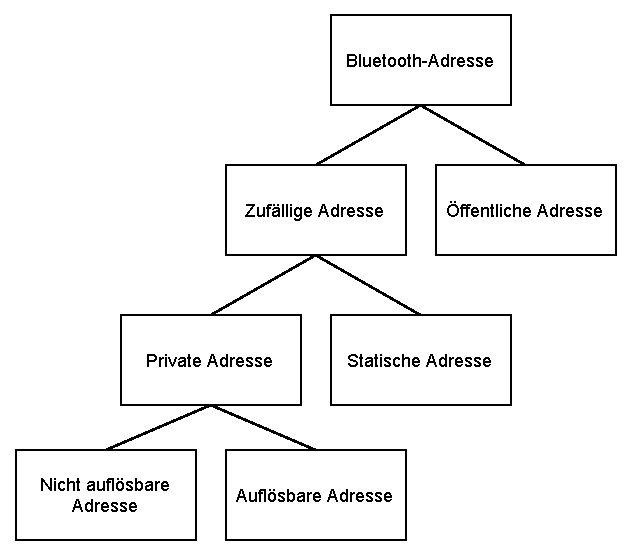
\includegraphics{graphics/BT_Adressen_Baum.pdf}
    \caption{Arten der Bluetooth-Adressen}
\end{figure}

Die öffentliche Bluetooth-Adresse ist die vom Hersteller bzw. IEEE festgelegte Adresse mit einer Länge von 48 Bit. Die 24 Bit mit dem höchsten Stellenwert bilden die von der IEEE vergebene Hersteller-ID und die 24 Bit mit dem niedrigsten Stellenwert bilden die vom Hersteller festgelegte Geräts-ID. \cite{BtSpec4.2_2576}
% QUELLE Spec. 4.2 S. 2576, 1.3.1 Public Device Address

Eine zufällig generierte Adresse kann entweder statisch oder privat sein. Eine zufällige statische Adresse kann bei jedem Neustart des Gerätes geändert werden und soll nicht während der Laufzeit geändert werden. Die zwei Bits mit dem höchsten Stellenwert sind jeweils auf 1 gesetzt, während die restlichen 46 Bit zufällig generiert werden, ohne dass alle nur auf 0 oder nur auf 1 gesetzt sind.

Zufällig generierte private Adressen werden in auflösbare und nicht auflösbare Adressen unterschieden. Eine Nicht auflösebare Adresse ist an den zwei Bit mit höchstem Stellenwert jeweils auf 0 gesetzt und die restlichen 46 Bit werden zufällig generiert, ohne dass alle nur auf 0 oder nur auf 1 gesetzt sind. Zudem darf diese Adresse nicht der öffentlichen Adresse gleichen.

Mittels eines IRK (der lokale oder der eines Peer-Geräts) und einer zufällig generierten Zahl (24 Bit Länge) kann ein Gerät eine auflösbare Adresse generieren. Die zwei Bit der zufällig generierten Zahl mit dem höchsten Stellenwert sind auf 0 (höchster Stellenwert) und 1 (zweithöchster Stellenwert) gesetzt, während die restlichen 22 Bit zufällig generiert werden, ohne dass alle nur auf 0 oder nur auf 1 gesetzt sind. Diese zufällig generierte Zahl nimmt die 24 Bit mit den höchsten Stellenwerten ein. Die restlichen 24 Bit mit den niedrigsten Stellenwerten der Adresse repräsentieren einen Hashwert, der mit der Funktion ah \cite{BtSpec4.2_2287} 
% QUELLE VERWEIS Spec. 4.2 S. 2287, 2.2.2 Random Address Hash function ah
und den Eingabewerten IRK und der zufällig generierten Zahl ermittelt wird. \cite{BtSpec4.2_2577-2579}
% QUELLE Spec. 4.2 S. 2577 -2579, 1.3.2 Random Device Address
\\\\

Nutzt ein Broadcaster oder Observer das Privacy Feature, dann verwendet er eine auflösbare oder nicht auflösbare Adresse, die er zeitlich periodisch ändert, solang er das Advertising bzw. Scanning betreibt. Jedoch wird die Adresse nur dann geändert, wenn der Controller die Auflösung von Adressen nicht unterstützt. Beim Advertising sollte der Broadcaster (genauso Peripherals) nicht seinen Gerätenamen oder Daten preisgeben, die zu dessen Identifikation verhelfen. \cite{BtSpec4.2_2078-2079}
% QUELLE Spec. 4.2 S. 2078 - 2079., 10.7.3 Privacy Feature in a Broadcaster, 10.7.4 Privacy Feature in an Observer

Ein Peripheral mit aktiviertem Privacy Feature nutzt im Connectable Mode eine auflösbare Adresse und im Non-Connectable Mode eine auflösbare oder nicht auflösbare Adresse. Empfängt das Peripheral eine auflösbare Adresse und verfügt über Bonding-Information, löst es mit diesen die empfangene Adresse auf. Konnte die empfangene Adresse erfolgreich aufgelöst werden, kann das Peripheral die Verbindung mit dieser akzeptieren. Anderenfalls wird die Verbindung abgelehnt oder das Pairing ausgeführt. Basiert das Privacy Feature des Peripheral auf dem Host, dann wird die auflösbare bzw. nicht auflösbare Adresse nur während des Advertising zeitlich periodisch geändert. \cite{BtSpec4.2_2077}
% QUELLE Spec. 4.2 S. 2077, 10.7.1 Privacy Feature in a Peripheral

Während des Scanning nutzt ein Central eine auflösbare oder nicht auflösebare Adresse, als Initiator dagegen nur eine auflösbare Adresse. Empfängt das Central eine auflösbare Adresse und verfügt über Bonding-Information, löst es mit diesen die empfangene Adresse auf. Konnte die empfangene Adresse erfolgreich aufgelöst werden, kann das Central die Verbindung mit dieser akzeptieren. Anderenfalls wird die enpfangene Adresse nicht beachtet. Basiert das Privacy Feature des Central auf dem Host, dann wird die auflösbare bzw. nicht auflösbare Adresse nur während des Scanning zeitlich periodisch geändert. \cite{BtSpec4.2_2078}
% QUELLE Spec. 4.2 S. 2078, 10.7.2 Privacy Feature in a Central